
\documentclass[10pt,twoside,reqno]{article}
\raggedbottom

\usepackage[bottom]{footmisc}		%% footnotes
\setlength{\footnotemargin}{0.6em}

\usepackage{blindtext}
\RequirePackage{setspace}
\RequirePackage{etoolbox}

\title{Supplementary Materials: Family structure and the well being of pregnant women in India, 2005-2021}

\date{}

%\usepackage[none]{hyphenat}		%% no hyphenation [!] if style errors occur, solve with \linebreak
\usepackage[utf8]{inputenc}			%% input-encoding: unicode

\makeatletter
\renewcommand*{\@pnumwidth}{3em} %% Width of the box for the page number in the TOC
\setlength{\@fptop}{0pt}				 %%	Floats to the top of the page
%\g@addto@macro\normalsize{%		 %% force equasion spacing to 10pt (font size); it can be helpful to increase the long skips to 12pt to fix spacing issues (of matrices in particular)
%  \setlength\abovedisplayskip{10pt}
%  \setlength\belowdisplayskip{10pt}
%  \setlength\abovedisplayshortskip{10pt}
%  \setlength\belowdisplayshortskip{10pt}
%}
\makeatother

\usepackage{printlen}
\uselengthunit{pt}
\usepackage[hidelinks]{hyperref}

%% inhaltsverzeichnis, überschriften
\usepackage{titlesec}
\titleformat{\section}[hang]{\raggedright\normalfont\bfseries\large}{\arabic{section}.}{1ex}{}
\titleformat{\subsection}[hang]{\raggedright\normalfont\bfseries}{\arabic{section}.\arabic{subsection}}{1ex}{}
\titleformat{\subsubsection}[hang]{\raggedright\normalfont\bfseries}{\arabic{section}.\arabic{subsection}.\arabic{subsubsection}}{1ex}{}



%% insert any additional packages and commands here
% Figures and captions
\usepackage{graphicx}
\graphicspath{{./figures/}}
\usepackage{caption}
\usepackage[font=scriptsize]{subcaption}
\captionsetup[figure]{labelsep=none}
\captionsetup[table]{labelsep=none}

% Math and symbols
\usepackage{amsmath}
\usepackage{bbm}
\usepackage{bm}
\usepackage{calc}

% Tables
\usepackage{array}
\usepackage{booktabs}
\usepackage{makecell}
\usepackage{tabularx}
\usepackage{longtable}
\usepackage{threeparttable}
\usepackage{siunitx}
\sisetup{detect-all}

% Colors
\usepackage[table]{xcolor}
\definecolor{Gray}{gray}{0.9}

% Layout and spacing
\usepackage[margin=1in]{geometry}
\usepackage{setspace}

\usepackage{indentfirst}
\usepackage{afterpage}
\usepackage{adjustbox}
\usepackage{pdflscape}
\usepackage{rotating}

% Floats
\usepackage{float}
\floatstyle{plaintop}
\restylefloat{table}
\usepackage{floatrow}
\usepackage{placeins}

% Text highlighting
\usepackage{soul}

% Bibliography and links
\usepackage[round]{natbib}
\setcitestyle{authoryear}


% Section/title and authors
\usepackage{titlesec}


% Importing files
\usepackage{import}

\newcommand\ddfrac[2]{\frac{\displaystyle #1}{\displaystyle #2}}

%%%%%%%%%%%%%%%%%%%%%%

\begin{document}

\onehalfspacing
%%%%%%%%%%%%%%%%%%%%%%%%%%%%%%%%%%%%%%%%%%%%%%%%%%%%%%%%%%%%%%%%%%%%%
%% do not change
\widowpenalty = 10000
\clubpenalty = 10000

\setlength{\parskip}{0ex}
\setlength{\parindent}{.7cm}
\setlength{\bibsep}{.18cm}
\setlength{\belowdisplayskip}{15pt} \setlength{\belowdisplayshortskip}{10pt}
\setlength{\abovedisplayskip}{15pt} \setlength{\abovedisplayshortskip}{10pt}


\maketitle
\thispagestyle{plain}


					
\maketitle
\thispagestyle{plain}


\section*{Appendix}
\addcontentsline{toc}{section}{\numberline{}Appendix}

% Appendix section labels: A, B, C, ...
\setcounter{section}{0}
\renewcommand{\thesection}{\Alph{section}}

% Appendix table/figure/equation labels: A-1, A-2, etc.
\setcounter{equation}{0}
\renewcommand{\theequation}{\thesection-\arabic{equation}}
\setcounter{figure}{0}
\renewcommand{\thefigure}{\thesection-\arabic{figure}}
\setcounter{table}{0}
\renewcommand{\thetable}{\thesection-\arabic{table}}

% ---------------------------------------------------------
% Appendix A
% ---------------------------------------------------------
\refstepcounter{section}
\subsection*{\thesection. Kitagawa decomposition of changes in family structure}
\label{sec:decomposition_parity}
We use Kitagawa decomposition \citep{kitagawa1955components} to assess whether the increase in the proportion of women living in patrilocal extended households observed between 2005--2006 and 2019--2021 in Table 1 in the main manuscript can be explained by compositional shifts in parity. 

For the proportion of women living in patrilocal extended households, $Y$, the change between NFHS-3 (2005--2006) and NFHS-5 (2019--2021) can be written as:

\begin{equation}
\Delta \equiv \bar Y^{5} - \bar Y^{3}
= \Delta_{\text{explained}} + \Delta_{\text{unexplained}}
\end{equation}

\begin{equation}
\Delta_{\text{explained}} =
\sum_{p \in \{1,2,3,4+\}} \big(s_p^{5} - s_p^{3}\big)\frac{Y_p^{5} + Y_p^{3}}{2}
\end{equation}

\begin{equation}
\Delta_{\text{unexplained}} =
\sum_{p \in \{1,2,3,4+\}} \big(Y_p^{5} - Y_p^{3}\big)\frac{s_p^{5} + s_p^{3}}{2}
\end{equation}



\begin{itemize}
    \item where $p \in \{1,2,3,4+\}$ indexes parity
    \item $\bar Y^{3}$ and $\bar Y^{5}$ are the proportion of pregnant women in patrilocal extended households in NFHS-3 (2005--2006) and NFHS-5 (2019--2021)
    \item $Y_p^{3}$ and $Y_p^{5}$ are the proportion of pregnant women in patrilocal extended households within parity $p$ in NFHS-3 (2005--2006) and NFHS-5 (2019--2021)
    \item $s_p^{3}$ and $s_p^{5}$ are the shares of pregnant women at parity $p$ in NFHS-3 (2005--2006) and NFHS-5 (2019--2021)
\end{itemize}

Table \ref{tab:decomposition_parity} shows the results of this decomposition. The distribution of pregnant women across parities explains 53\% of the increase in patrilocal residence among pregnant women between 2005 and 2021. In 2005--2006, more than a quarter of pregnant women had three or more prior live births, compared to only 11\% in 2019--2021. Patrilocal residence is also higher at lower parities, with more than three quarters of pregnant women living in patrilocal households in both survey rounds. This may reflect a life course theory of household structure that ties nuclear residence to family size. Or, higher parity may be capturing other determinants of nuclear residence in the life course, such as better financial status, older ages, or living parents -- The sample of pregnant women in 2019--2021 consisted of less women at later parities with these characteristics compared to 2005--2006, which may explain the higher observed patrilocal residence. 

\begin{table}[H]
\sffamily
\caption{: More than half of the increase in patrilocal extended household residence among pregnant women between 2005--2006 and 2019--2021 can be explained by lower parities in 2019--2021}
\label{tab:decomposition_parity}
\vspace{-4pt}

\begin{center}
\begin{scriptsize}
\begin{adjustbox}{max width=\textheight, max totalheight=\textwidth, keepaspectratio}
\setlength{\tabcolsep}{4pt}
\renewcommand{\arraystretch}{1.3}
\begin{tabular}{>{\raggedright\arraybackslash}p{1.8cm}>{\centering\arraybackslash}p{1.25cm}>{\centering\arraybackslash}p{1.25cm}>{\centering\arraybackslash}p{1.45cm}>{\centering\arraybackslash}p{1.45cm}>{\centering\arraybackslash}p{1.45cm}>{\centering\arraybackslash}p{1.45cm}}
\toprule
Parity group & \makecell{Parity\\share\\2005--2006\\(\%)} & \makecell{Parity\\share\\2019--2021\\(\%)} & \makecell{Patrilocal\\share\\2005--2006\\(\%)} & \makecell{Patrilocal\\share\\2019--2021\\(\%)} & \makecell{Explained\\change\\share\\(\%)} & \makecell{Unexplained\\change\\share\\(\%)} \\
\midrule
Parity 0&29.62&39.35&78.24&84.24&76.95&20.15\\
Parity 1&28.45&33.88&64.92&70.79&35.86&17.82\\
Parity 2&16.59&15.48&55.16&59.92&-6.25&7.43\\
Parity 3+&25.34&11.30&38.60&39.34&-53.28&1.32\\
Total&100.00&100.00&60.58&70.85&53.28&46.72\\
\bottomrule
\end{tabular}

\end{adjustbox}
\end{scriptsize}
\end{center}

\vspace{1ex}
\small\scriptsize{\textsf{\textit{Note}: Data are from the NFHS rounds 3 (2005--2006), 4 (2015--2016), and 5 (2019--2021).}}
\newline\small\scriptsize{\textsf{Parity refers to the number of prior live births at the time of the interview.  The current pregnancy is therefore not counted.}}
\newline\small\scriptsize{\textsf{The sample is restricted to ever-married women who report being three or more months pregnant at the time of the survey, and who live in either nuclear or patrilocal extended household structures. Women reporting early pregnancy (one to two months) are excluded because early detection is selective, as shown in Table \ref{tab:earlypregnancy}. }}

\end{table}


% ---------------------------------------------------------
% Appendix B
% ---------------------------------------------------------
\clearpage
\renewcommand{\thesection}{B-\arabic{section}}
\setcounter{equation}{0}
\renewcommand{\theequation}{B-\arabic{equation}}
\setcounter{figure}{0}
\renewcommand{\thefigure}{B-\arabic{figure}}
\setcounter{table}{0}
\renewcommand{\thetable}{B-\arabic{table}}

\refstepcounter{section}
\subsection*{B. Justification of decision to drop women reporting one or two months of pregnancy} \label{sec:dropearlypregnancy}

The main sample of pregnant women used in the paper excludes those who report being one or two months pregnant at the time of the survey, 
to avoid biasing the results due to selection into early detection and reporting of pregnancy.

To confirm that the sample of women who report being one or two months pregnant is systematically different than those reporting three or more months of 
pregnancy, we estimate the following linear probability regression on the entire sample of women who report being currently pregnant:

\begin{equation}
Y_i=X_i B+\epsilon_i
\end{equation}

where for woman $i$, 
\begin{itemize}
    \item $Y_i$ is an indicator for reporting one or two months of pregnancy (as opposed to three or more)
    \item $X_i$ is a set of indicators for less than primary education, rural residence, whether the woman does not have any sons, 4 age bins, 10 parity and time since last birth categories, and wealth quartiles. 
\end{itemize}

We report the estimated coefficients $B$ in Table \ref{tab:earlypregnancy} to check the balance of variables in $X_i$ across women reporting one or two months of pregnancy and women reporting three or more. Because the models are linear probability models, coefficients can be interpreted as percentage-point differences in the probability of reporting one or two months of pregnancy relative to the omitted category. The coefficients suggest that women who report being one or two months pregnant are systematically different from women reporting later pregnancy, though the differences are modest. Across survey rounds, women aged 20 and older are less likely than women aged 15--19 to report being one or two months pregnant, indicating that early pregnancy reports are concentrated among younger pregnant women. In some rounds, women in higher wealth quartiles are more likely to report early pregnancy, while differences by rural residence, son status, parity, and social group are less consistent across rounds. These patterns support our decision to exclude women reporting one or two months of pregnancy from the main analytic sample of pregnant women.

\begin{table}[H]
\sffamily
\caption{: Women reporting one or two months of pregnancy differ from women reporting later pregnancy}
\label{tab:earlypregnancy}
\vspace{-8pt}

\begin{center}
\begin{scriptsize}
\setlength{\tabcolsep}{10pt}
\renewcommand{\arraystretch}{0.9}
\begin{adjustbox}{max width=\textwidth, max totalheight=0.86\textheight, keepaspectratio}
\begin{tabular}{l*{3}{c}}
\toprule
                    &\multicolumn{3}{c}{reports of 1 or 2 months of pregnancy}\\\cmidrule(lr){2-4}
                    &\multicolumn{1}{c}{2005-2006}&\multicolumn{1}{c}{2015-2016}&\multicolumn{1}{c}{2019-2021}\\
\midrule
\hspace*{1em}Less than primary education&       0.002&      -0.019&      -0.002\\
                    &    (0.0140)&    (0.0061)&    (0.0067)\\
\addlinespace
\hspace*{1em}Rural resident&      -0.001&       0.011&       0.008\\
                    &    (0.0136)&    (0.0075)&    (0.0084)\\
\addlinespace
\hspace*{1em}Does not have boy child&      -0.008&       0.009&      -0.003\\
                    &    (0.0134)&    (0.0066)&    (0.0072)\\
\addlinespace
\textbf{Age categories} \\ (15--19 omitted)&            &            &            \\
\addlinespace
\hspace*{1em}20--24 &      -0.035&      -0.034&      -0.024\\
                    &    (0.0171)&    (0.0095)&    (0.0098)\\
\addlinespace
\hspace*{1em}25--29 &      -0.048&      -0.039&      -0.032\\
                    &    (0.0195)&    (0.0110)&    (0.0115)\\
\addlinespace
\hspace*{1em}30--49 &      -0.051&      -0.041&      -0.010\\
                    &    (0.0228)&    (0.0134)&    (0.0177)\\
\addlinespace
\textbf{Parity (live births)} \\ (0 omitted)&            &            &            \\
\addlinespace
\hspace*{1em}1      &       0.013&      -0.009&      -0.003\\
                    &    (0.0147)&    (0.0074)&    (0.0088)\\
\addlinespace
\hspace*{1em}2      &      -0.007&       0.003&      -0.003\\
                    &    (0.0197)&    (0.0097)&    (0.0106)\\
\addlinespace
\hspace*{1em}3+     &      -0.005&       0.024&      -0.009\\
                    &    (0.0209)&    (0.0128)&    (0.0139)\\
\addlinespace
\textbf{Wealth quartiles} \\ (1st quartile omitted)&            &            &            \\
\addlinespace
\hspace*{1em}2nd quartile&       0.018&       0.012&       0.011\\
                    &    (0.0153)&    (0.0073)&    (0.0076)\\
\addlinespace
\hspace*{1em}3rd quartile&       0.014&       0.021&       0.009\\
                    &    (0.0171)&    (0.0090)&    (0.0093)\\
\addlinespace
\hspace*{1em}4th quartile&       0.042&       0.023&       0.003\\
                    &    (0.0234)&    (0.0110)&    (0.0116)\\
\addlinespace
\textbf{Social group} \\ (Adivasi omitted)&            &            &            \\
\addlinespace
\hspace*{1em}Dalit  &      -0.002&      -0.021&       0.003\\
                    &    (0.0201)&    (0.0099)&    (0.0105)\\
\addlinespace
\hspace*{1em}OBC    &       0.017&      -0.012&       0.000\\
                    &    (0.0194)&    (0.0092)&    (0.0098)\\
\addlinespace
\hspace*{1em}Forward caste&      -0.005&      -0.006&       0.007\\
                    &    (0.0214)&    (0.0117)&    (0.0159)\\
\addlinespace
\hspace*{1em}Muslim &      -0.014&       0.001&       0.007\\
                    &    (0.0206)&    (0.0116)&    (0.0117)\\
\addlinespace
\hspace*{1em}Constant&       0.125&       0.158&       0.145\\
                    &    (0.0317)&    (0.0159)&    (0.0167)\\
\midrule
\textbf{N}          &       5,693&      31,835&      27,939\\
\bottomrule
\end{tabular}

\end{adjustbox}
\end{scriptsize}
\end{center}

\vspace{0.5ex}
\vspace{0.5ex}
\small\scriptsize{\textsf{\textit{Note}: Data are from NFHS rounds 3 (2005--2006), 4 (2015--2016), and 5 (2019--2021). Coefficients are from weighted linear probability models estimated separately by survey round. The dependent variable is an indicator for reporting one or two months of pregnancy among women who report being currently pregnant. Brackets report 95\% confidence intervals. Models include state fixed effects, and standard errors are clustered at the primary sampling unit level.}}
\newline\small\scriptsize{\textsf{The sample includes all women who self-report being pregnant at the time of the survey.}}
\newline\small\scriptsize{\textsf{Gestational duration is defined using the reported number of months since the start of the woman's last menstrual period. If that was not reported, we use her answer to the question, ``How many months pregnant are you?'' This substitution is made for 5\% of women who report being currently pregnant.}}
\end{table}

% ---------------------------------------------------------
% Appendix C
% ---------------------------------------------------------
\clearpage

% Appendix C: section reference should be just C
\renewcommand{\thesection}{C}

% Appendix C: figures/tables/equations should be C-1, C-2, etc.
\setcounter{equation}{0}
\renewcommand{\theequation}{C-\arabic{equation}}

\setcounter{figure}{0}
\renewcommand{\thefigure}{C-\arabic{figure}}

\setcounter{table}{0}
\renewcommand{\thetable}{C-\arabic{table}}

% Make the label point to C
\refstepcounter{section}
\subsection*{C. Distribution of women by household type in NFHS-2005, 2015, and 2021}
\label{appendix:hhstructure}

The sample used for the main analysis in this paper focuses on pregnant women aged 15--49 who live in either nuclear or patrilocal extended household structures, excluding women living in natal households.

Figure \ref{fig:bargraph} shows the composition of household structure in different samples of women aged 15--49. While the main analysis in the paper focuses on pregnant women, trends of increasing patrilocal extended residence are also present in the sample of nonpregnant women, and the sample used in \cite{allendorf2013going}. 

In all samples shown in Figure \ref{fig:bargraph} except the sample used in \cite{allendorf2013going}, the bar graph keeps the subsample of women in natal households to show that its proportion remains stable over time, and that its exclusion does not affect trends in nuclear and patrilocal extended household structures.


\begin{figure}[H]
\begin{flushleft}
\captionsetup{style=CAPFIG}
\caption{The proportion who reside in natal households remains similar over time in relevant sub-samples of women}
\label{fig:bargraph}
\vspace{0em}

\begin{center}
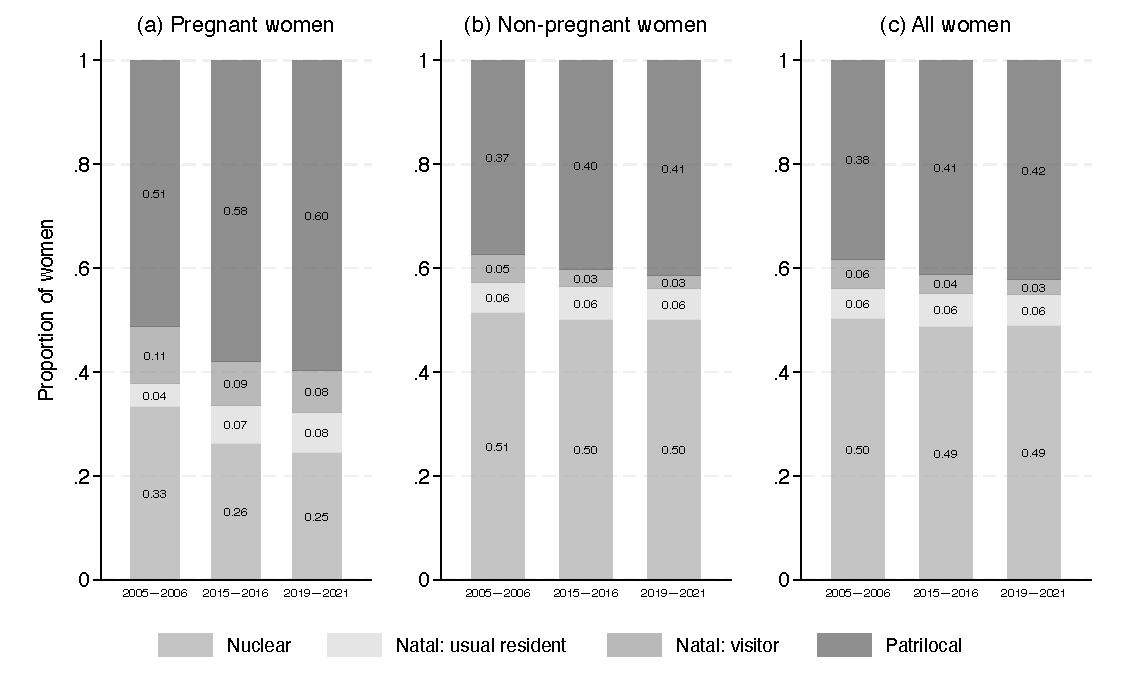
\includegraphics[scale=0.6]{figures/figureC1_hhstruc_composition_allwomen.pdf}
\end{center}

\vspace{1ex}
\small\scriptsize{\textsf{\textit{Note}: Data are from the NFHS rounds 3 (2005--2006), 4 (2015--2016), and 5 (2019--2021). Panel (a) uses the sample of ever-married women who report being three or more months pregnant at the time of the survey. Panel (b) uses the sample of ever-married women who do not report being pregnant at the time of the survey. Panel (c) has all ever married women 15--49. All panels drop women in their respective samples who are not in either nuclear, natal, or patrilocal households.}}

\end{flushleft}
\end{figure}


Figure \ref{fig:hh_structure_men} shows trends in household structure among men whose wives were pregnant at the time of the survey. As seen in Figure \ref{fig:bargraph}, the majority of pregnant women in natal households are visitors -- this may be because women temporarily return to their natal households during pregnancy. It would shed doubt on our observation of increasing patrilocal residence if it was the case that the pregnant women who are observed as visitors in natal households were predominantly from patrilocal households in 2005--2006, but were predominantly from nuclear households in 2019--2021. To test this, we observe changes in household structure based on the sample of men married to a woman who is currently pregnant. In the case that pregnant women visit their natal households alone without their husbands, this allows us to observe changes in the usual household structure of women. 


\begin{figure}[H]
\begin{flushleft}
\caption{: Household structure among married men whose wives are currently pregnant}
\label{fig:hh_structure_men}
\vspace{0em}
\begin{center}
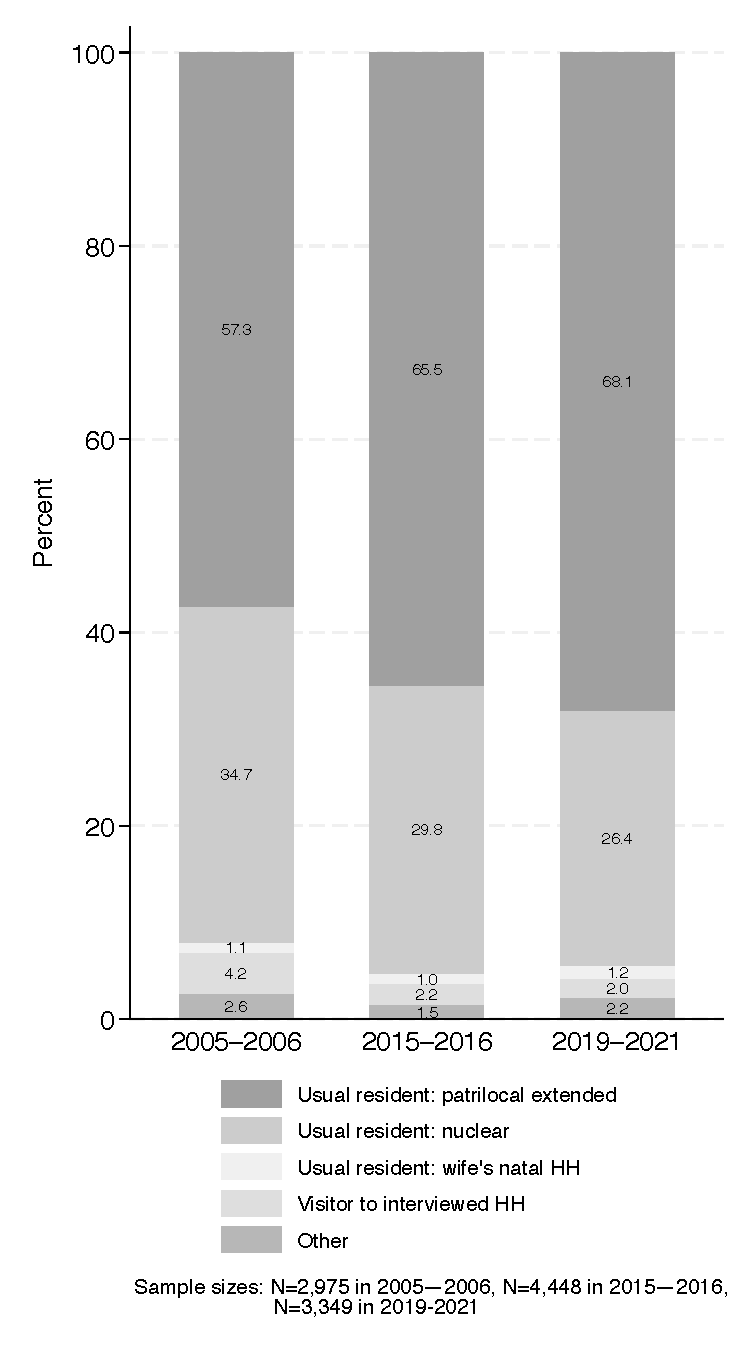
\includegraphics[width=0.5\textwidth]{figures/figureC2_hhstruc_composition_husbands.pdf}
\end{center}
\vspace{1ex}
\small\scriptsize{\textsf{\textit{Note}: Data are from NFHS rounds 3 (2005--2006), 4 (2015--2016), and 5 (2019--2021). The sample is restricted to currently married men whose wife was pregnant at the time of the survey and who live in one of the household structures included in the figure. Household structure is defined from the perspective of each man's wife, following the description in the Variables section in the main text.}}
\end{flushleft}
\end{figure}




% ---------------------------------------------------------
% Appendix D
% ---------------------------------------------------------
\clearpage
\renewcommand{\thesection}{D-\arabic{section}}
\setcounter{equation}{0}
\renewcommand{\theequation}{D-\arabic{equation}}
\setcounter{figure}{0}
\renewcommand{\thefigure}{D-\arabic{figure}}
\setcounter{table}{0}
\renewcommand{\thetable}{D-\arabic{table}}

\refstepcounter{section}
\subsection*{D. Kitagawa decomposition of changes in autonomy and healthcare indicators} \label{sec:decomposition_outcomes}

To assess whether changes in autonomy and maternal healthcare are driven by shifts in the distribution of household structure or by changes within household types, we implement a Kitagawa decomposition \citep{kitagawa1955components} comparing NFHS-3 (2005--2006) and NFHS-5 (2019--2021), using NFHS-3 as the baseline.

For each outcome $Y$ (no say in own healthcare, no say in visits to family/friends, four or more prenatal visits, birth in a health facility), the change between NFHS-3 (2005--2006) and NFHS-5 (2019--2021) can be written as:

\begin{equation}
\Delta \equiv \bar Y^{5} - \bar Y^{3}
= \Delta_{\text{explained}} + \Delta_{\text{unexplained}}
\end{equation}

\begin{equation}
\Delta_{\text{explained}} =
\sum_{j \in \{N,P\}} \big(p_j^{5} - p_j^{3}\big)\frac{Y_j^{5} + Y_j^{3}}{2}
\end{equation}

\begin{equation}
\Delta_{\text{unexplained}} =
\sum_{j \in \{N,P\}} \big(Y_j^{5} - Y_j^{3}\big)\frac{p_j^{5} + p_j^{3}}{2}
\end{equation}

\begin{itemize}
    \item $j \in \{N,P\}$ indexes household type: nuclear ($N$) and patrilocal ($P$)
    \item $\bar Y^{3}$ and $\bar Y^{5}$ are the mean outcomes in NFHS-3 (2005--2006) and NFHS-5 (2019--2021)
    \item $Y_j^{3}$ and $Y_j^{5}$ are the mean outcomes within household type $j$ in NFHS-3 (2005--2006) and NFHS-5 (2019--2021)
    \item $p_j^{3}$ and $p_j^{5}$ are the proportions of women residing in household type $j$ in NFHS-3 (2005--2006) and NFHS-5 (2019--2021)
\end{itemize}


Appendix Table \ref{tab:decomposition_outcomes} shows results from this decomposition. All four outcomes (no say in own healthcare, no say in visits to family/friends, four or more prenatal visits, birth in a health facility) have improved between 2005 and 2021. Pregnant women in 2019--2021 are 23 percentage points less likely to report having no say in their own healthcare, and 28 percentage points less likely to report having no say in visits to family or friends. Women who gave birth in the 3--12 months before the survey were 22 percentage points more likely to have had four or more prenatal visits, and 50 percentage points more likely to have given birth in a health facility. 

\begin{table}[H]
\sffamily
\caption{: None of the improvement in the outcomes is explained by changing composition in household structures}
\label{tab:decomposition_outcomes}
\vspace{-4pt}

\begin{scriptsize}
\setlength{\tabcolsep}{4pt}
\renewcommand{\arraystretch}{2.5}

\makebox[\linewidth][c]{%
\begin{tabular}{lccc}
\toprule
Outcome & \makecell{Total change\\(pp)} & \makecell{Share explained by \\household structure (\%)} & \makecell{Share from within-\\household structure changes (\%)} \\
\midrule
No say in own healthcare$^1$&-23.22&-5.15&105.15\\
No say in visits to family/friends$^1$&-27.96&-5.27&105.27\\
Four or more prenatal visits$^2$&22.20&3.25&96.75\\
Birth in a health facility$^2$&50.11&1.51&98.49\\
\bottomrule
\end{tabular}
%
}

\end{scriptsize}

\vspace{1ex}
\small\scriptsize{\textsf{\textit{Note}: Data are from NFHS rounds 3 (2005--2006), 4 (2015--2016), and 5 (2019--2021).}}
\newline
\small\scriptsize{\textsf{$^1$ The sample is restricted to ever-married women who report being three or more months pregnant at the time of the survey, and who live in either nuclear or patrilocal extended households.}}
\newline
\small\scriptsize{\textsf{$^2$ The sample is restricted to ever-married women who report having given birth in the last 3--12 months, and who live in either nuclear or patrilocal extended households.}}

\end{table}

%%%%%%%%%%%%%%%%%%%%%% END APPENDIX %%%%%%%%%%%%%%%%%%%%%%%%%%

% Ensure that there is an even number of pages. 
\cleardoublepage

\bibliographystyle{DemRes}
\bibliography{references_DR_format} % bibliography file

\end{document}


